\documentclass[12pt,a4paper,english]{article}
\usepackage{times}
\usepackage[utf8]{inputenc}
\usepackage{babel,textcomp}
\usepackage{mathpazo}
\usepackage{mathtools}
\usepackage{amsmath,amssymb}
\usepackage{ dsfont }
\usepackage{listings}
\usepackage{graphicx}
\usepackage{float}
\usepackage{subfig} 
\usepackage[colorlinks]{hyperref}
\usepackage[usenames,dvipsnames,svgnames,table]{xcolor}
\usepackage{textcomp}
\definecolor{listinggray}{gray}{0.9}
\definecolor{lbcolor}{rgb}{0.9,0.9,0.9}
\lstset{backgroundcolor=\color{lbcolor},tabsize=4,rulecolor=,language=python,basicstyle=\scriptsize,upquote=true,aboveskip={1.5\baselineskip},columns=fixed,numbers=left,showstringspaces=false,extendedchars=true,breaklines=true,
prebreak=\raisebox{0ex}[0ex][0ex]{\ensuremath{\hookleftarrow}},frame=single,showtabs=false,showspaces=false,showstringspaces=false,identifierstyle=\ttfamily,keywordstyle=\color[rgb]{0,0,1},commentstyle=\color[rgb]{0.133,0.545,0.133},stringstyle=\color[rgb]{0.627,0.126,0.941},literate={å}{{\r a}}1 {Å}{{\r A}}1 {ø}{{\o}}1}

% Use for references
\usepackage[sort&compress,square,comma,numbers]{natbib}
\DeclareRobustCommand{\citeext}[1]{\citeauthor{#1}~\cite{#1}}

% Fix spacing in tables and figures
%\usepackage[belowskip=-8pt,aboveskip=5pt]{caption}
%\setlength{\intextsep}{10pt plus 2pt minus 2pt}

% Change the page layout
%\usepackage[showframe]{geometry}
\usepackage{layout}
\setlength{\hoffset}{-0.5in}  % Length left
%\setlength{\voffset}{-1.1in}  % Length on top
\setlength{\textwidth}{470pt}  % Width
%\setlength{\textheight}{720pt}  % Height
%\setlength{\footskip}{25pt}

\newcommand{\VEV}[1]{\langle#1\rangle}
\title{FYS-STK 4155 Project 1}
\date{}
\author{ Kristoffer Langstad \footnote{\url{https://github.com/krilangs/FYS-STK4155}}\\ \textit{krilangs@uio.no}}

\begin{document}%layout
\maketitle
\begin{abstract}
In this project, we want to analyze different linear regression models on two different given data sets.  First we will analyze what is called the Franke function with an added stochastic noise following a normal distribution, and then we will analyze real digital terrain data. The Franke function only contains about 400 data points, while the full digital terrain data contains about 6.5million data points. Our computer can't handle such big data sets, so we have to reduce it to be able to analyze the data set. To analyze these data sets, we will use three different regression models; the Ordinary Least Squares (OLS) method, Ridge regression and Lasso regression. We will fit these models to the mentioned data sets as polynomials of varying degree. These regression methods are then combined with with the k-fold cross-validation resampling method for splitting the data set into a training set and a test set. Then we can evaluate the errors and the evaluation scores to see how well fitted our models are to the data sets depending on the model complexity and hyperparameters. We will also look at the bias-variance tradeoff we get as the complexity increases. From theory we could expect that the OLS would be the best fit model. This arises from the fact that Ridge and Lasso have a shrinking parameter, $\lambda$, that pushes the regression parameters, $\beta$, towards zero. As $\lambda$ gets closer to zero, we would expect the solutions to go towards the same as for the OLS model. From our results on the Franke function with a noise term with standard deviation $\sigma=0.2$, we can conclude that this happens. We get the smallest Mean Squared Error (MSE) and the best $R^2$ score from the OLS method for dimension 9 with $MSE=0.040959$ and $R^2=0.680520$. The results for Ridge and Lasso are close to the OLS results for very low $\lambda$'s ($\approx 10^{-7}$) with the same dimensionality.
\end{abstract}

\section{Introduction}
A hot topic today is what we call machine learning. We use machine learning to analyze data (often a huge amount). There are now many different methods for doing this, where some are better than others in different cases. A way to study machine learning is to look at regression analysis and resampling methods of given data sets, which is split into what we call training and test data. Then we can study the data dependence and the effect of different hyper-parameters.

We will in this project study three linear regression methods: the Ordinary Least Squares (OLS), Ridge regression and Lasso regression. In linear regression we will fit a polynomial to a given data set that we want to analyze. Linear regression let use look at relationships in data sets that are normally hidden under complexities and huge quantities of data. In our case we will first fit a polynomial to a two-dimensional function called Franke's function (which we will look at later). After implementing the regression methods we will use resampling techniques, like cross-validation, to perform a more thorough assessment of the models we have. Then we can also look at the Bias-Variance tradeoff as we look at a varying model complexity of the data set and models. Lastly we will use all the techniques we have mentioned to analyze real data terrain to see which model and degree of polynomial has the best fit.

In the methods section we look at the theory of the different models, techniques and the implementations of the algorithms we use in this project. We start by looking at the OLS of the Franke function where we use the Franke function, with and without an additional normally distributed stochastic noise, to produce a dataset to study with OLS regression. Then we want to fit a polynomial up to fifth order, and study the confidence interval of $\beta$ by computing the Mean Squared Error (MSE), $R^2$ score function and variance. Then we perform a resampling of the data where we split the data into training and test data. Then we construct the k-fold cross-validation algorithm and evaluate the MSE, $R^2$ score, variance and bias of the test data. For further studying machine learning, we study the bias and variance tradeoff as function of model complexity and number of data points. Now we have all the techniques we are using, so now we use the same techniques on the Ridge and Lasso method. For these two methods there is a hyperparameter dependence which we will also study. Then we want to introduce real terrain data to analyze. We use all three of the linear regression methods to evaluate which model fits the data best. In the Results section we look at the results and discuss all the methods and techniques used in this project. Here we look at data outputs and figures we get underway. Lastly in the Conclusion section we summarize the results and come up our thoughts on which model is the best fit for the terrain data.

\section{Theory}
\subsection{Linear regression}
In linear regression we want to fit a model to a set of data. For fitting a model to a set of data $\textbf{y}=[y_0, y_1,...,y_{n-1}]$ of length $n$ which are functions of some variables $\textbf{x}=[x_0, x_1,...,x_{n-1}]$. We can then define the prediction value $y$ as
\begin{equation}
\label{eq:pred_y}
y(x_i)=y_i=f(\cdot)+\epsilon_i=\sum_{n-1}^{i=0}\beta_jx_i^j+\epsilon_i,
\end{equation}
where $\beta$ are regression parameters and $\epsilon_i$ is a normally distributed error with mean zero and variance $\sigma^2$. The goal is to find the optimal regression parameters $\beta$. This can be done with different methods like OLS, Ridge and Lasso.

\subsection{Ordinary Least Square (OLS)}
In OLS we find the $\beta$ values that minimize the residual sum of squares (RSS), which here is a cost function dependent on the given data $y_i$ (data) and the parametrized values $\tilde{\textbf{y}}_i=\textbf{X}\hat{\beta}$ (model):
\begin{equation}
\label{eq:cost_OLS}
C(\hat{\beta})=\frac{1}{n}\sum_{i=0}^{n-1}(y_i-\tilde{y}_i)^2=\frac{1}{n}\sum_{i=0}^{n-1}(y_i-\textbf{x}_{i*}\hat{\beta})^2=\frac{1}{n}\{(\textbf{y}-\textbf{X}\hat{\beta})^T(\textbf{y}-\textbf{X}\hat{\beta})\}
\end{equation} 
\textbf{X} is our design matrix which contains the predictors. Then to find the minimum of the cost function we set $\frac{\partial C}{\partial \hat{\beta}}=0$ and solve
\[\min_{\hat{\beta}\in \mathcal{R}^p}C(\hat{\beta}).\] This should give us the optimal $\beta$ values as
\begin{equation}
\label{eq:beta_OLS_opt}
\hat{\beta}_{\text{optimal}}^{\text{OLS}}=(\textbf{X}^T\textbf{X})^{-1}\textbf{X}^T\textbf{y}
\end{equation}
These $\beta$ values are the model values in the OLS model.

Taking the inverse of a matrix product (\textbf{X}$^T$\textbf{X})$^{-1}$ may be an expensive operation for bigger matrices. That is why we take use of the Singular Value Decomposition (SVD) to prevent taking the inverse of the product of twp big matrices. From the SVD theorem we can expand our design matrix as:
\[\textbf{X}=\textbf{U}\textbf{D}\textbf{V}^T\]
This is written in terms of the orthogonal transformation \textbf{U}, the diagonal matrix \textbf{D} containing the eigenvalues and \textbf{V}$^T$ which is also an orthogonal matrix. By inserting this into the OLS we get:
\begin{equation}
\label{eq:beta_SVD_OLS}
\tilde{\textbf{y}}=\textbf{X}\hat{\beta}_{\text{optimal}}^{\text{OLS}}=\textbf{U}\textbf{U}^T\textbf{y}
\end{equation}
This is now a more CPU friendly calculation of the OLS for finding the regression parameters $\hat{\beta}$.

\subsection{Ridge regression}
A problem with machine learning  and regression is overfitting of the data when the model complexity increases. The Ridge regression tries to take this into account by modification of the OLS method by introducing a complexity parameter $\lambda$, also called the ad-hoc fix for singularity of \textbf{X}$^T$\textbf{X} (\citet{wieringen2015}). The Ridge method shrinks the coefficients $\beta$ to go to zero as $\lambda$ increases. The complexity parameter is a parameter that controls the amount of shrinkage of the coefficients (\citet{hastie2009}). The cost function for Ridge can then be written as
\begin{equation}
\label{eq:cost_ridge}
C(\hat{\beta})=\frac{1}{n}\sum_{i=0}^{n-1}(y_i-\textbf{x}_{i*}\hat{\beta})^2+\lambda\sum_{j=0}^{p-1}\beta_j^2=\frac{1}{n}\{(\textbf{y}-\textbf{X}\hat{\beta})^T(\textbf{y}-\textbf{X}\hat{\beta})\}+\lambda\hat{\beta}^T\hat{\beta}.
\end{equation}
The last term above is called the penalty term.
Then to find the optimal $\beta$ values we again take the minimum of the cost function to get
\begin{equation}
\label{eq:beta_opt_ridge}
\hat{\beta}_{\text{optimal}}^{\text{Ridge}}=(\textbf{X}^T\textbf{X}+\lambda \textbf{I})^{-1}\textbf{X}^T\textbf{y},
\end{equation}
where \textbf{I} is the identity matrix with dimension $p\times p$ and $\lambda\geq0$. For orthonormal matrix (which we get when using the SVD in the OLS method) we get \textbf{X}$^T$\textbf{X}=\textbf{I} and
\begin{equation*}
\hat{\beta}^{\text{Ridge}}=\frac{1}{1+\lambda}\hat{\beta}^{\text{OLS}}
\end{equation*}
We see that for $\lambda=0$ we end up with the expression for the OLS method, and since $\lambda$ is defined to never be negative we get that the $\beta$ values are smaller than for the OLS. This will make the model less sensitive to data set changes and making it less likely to overfit the training data. The model now should give a decrease in variance as the $\lambda$ increases, but then in return give an increase in the bias.

\subsection{Lasso regression}
The Lasso method is similar to the Ridge method in that case it has a complexity parameter $\lambda$, but now we change the penalty term in the cost function equation \ref{eq:cost_ridge}:
\begin{equation}
\label{eq:cost_lasso}
C(\hat{\beta})=\frac{1}{n}\sum_{i=0}^{n-1}(y_i-\textbf{x}_{i*}\hat{\beta})^2+\lambda\sum_{j=0}^{p-1}|\beta_j|
\end{equation}
A difference with the Lasso is that it uses methods like gradient descent to find the $\hat{\beta}$ that minimize the cost function. For the Lasso there is no explicit expression for the model parameters like for the OLS and Ridge methods. In this project we will just use Scikit-Learn's Lasso function, instead of making our own which can be difficult. The equation for the regression parameters is:
\begin{equation}
\label{eq:beta_opt_Lasso}
\hat{\beta}_{\text{optimal}}^{\text{Lasso}}=\min_{\hat{\beta}\in \mathcal{R}^p}\left[\frac{1}{n}\sum_{i=0}^{n-1}(y_i-\textbf{x}_{i*}\hat{\beta})^2+\lambda\sum_{j=0}^{p-1}|\beta_j|\right]
\end{equation} 
Like the Ridge method the task is to make the $\beta$ values go to zero, but in a slightly different way. So the variance should decrease while the bias should increase with increasing $\lambda$ also here.

\subsection{Confidence interval}
For the confidence interval of the parameters $\beta$ we need to calculate the variance of the models. The variance of the OLS model can be calculated as
\begin{equation}
\label{eq:var_ols}
Var(\hat{\beta})=\sigma^2(\textbf{X}^T\textbf{X})^{-1},
\end{equation}
where $\sigma^2$ is the variance of the normally distributed error $\epsilon_i$ in equation \ref{eq:pred_y}. This variance can be calculated as
\begin{equation}
\label{eq:sigma}
\sigma^2 = \frac{1}{n-p-1}\sum_{i=0}^{n-1}(y_i-\tilde{y}_i)^2.
\end{equation}
In \citet{hastie2009}\footnote{Chapter 3 - equation (3.14)} it is shown that the confidence interval of $\beta_j$ can be calculated as 
\begin{equation}
\label{eq:conf_int}
(\hat{\beta}_j-z^{(1-\alpha)}v_j^{\frac{1}{2}}\hat{\sigma}, \hat{\beta}_j+z^{(1-\alpha)}v_j^{\frac{1}{2}}\hat{\sigma})
\end{equation}
For a 95\% confidence interval we have $\alpha=0.05$ such that we get $z^{(1-0.05)}=1.96$. $v_j$ is the $j$-th diagonal element of (\textbf{X}$^T$\textbf{X})$^{-1}$.

\subsection{Error evaluation}
Two very useful tools for evaluating the error in predicted values are the Mean Squared Error (MSE) and the $R^2$ score function. The MSE is calculated as 
\begin{equation}
\label{eq:MSE}
MSE(\textbf{y}, \tilde{\textbf{y}})=\frac{1}{n}\sum_{i=0}^{n-1}(y_i-\tilde{y})^2,
\end{equation}
and the $R^2$ score function is calculated as
\begin{equation}
\label{eq:R2_score}
R^2(\textbf{y},\tilde{\textbf{y}})=1-\frac{\sum_{i=0}^{n-1}(y_i-\tilde{y})^2}{\sum_{i=0}^{n-1}(y_i-\bar{y})^2}
\end{equation}
with the mean value of the data $y$ as
\[\bar{y}=\frac{1}{n}\sum_{i=0}^{n-1}y_i.\]
$\textbf{y}_i$ is the predicted value of the $i$-th sample and $y_i$ is the corresponding true value of the data. For the MSE we want the error to be as small as possible, close to zero. For the $R^2$ score, the best value we can get is 1. This can be described as how much variance in the data is accounted for by the model. For a score of 1 means that the prediction fits the data perfect. The score can lie in the interval $(-\infty,1]$, meaning that the score can be negative. This can be interpreted such that the mean is a better fit than the model used.

\subsection{Bias-variance tradeoff}
To find the regression parameters $\hat{\beta}$ we have to look at the cost function again:
\begin{equation}
\label{eq:cost_func}
C(\textbf{X},\hat{\beta})=\frac{1}{n}\sum_{i=0}^{n-1}(y_i-\tilde{y}_i)^2= \mathds{E}[(\textbf{y}-\tilde{\textbf{y}})^2]
\end{equation}
This can be rewritten as 
\begin{equation}
\label{eq:bias_var}
\mathds{E}[(\textbf{y}-\tilde{\textbf{y}})^2]= \frac{1}{n}\sum_{i}(f_i-\mathds{E}[\tilde{\textbf{y}}])^2+ \frac{1}{n}\sum_{i}(\tilde{y}_i-\mathds{E}[\tilde{\textbf{y}}])^2+\sigma^2.
\end{equation}
The full calculation can be found in appendix \ref{sect:bias_var_calc}.

From the rewritten cost function we now have three terms in the equation above. The first term is the bias squared
\begin{equation}
\label{eq:Bias}
Bias=\frac{1}{n}\sum_{i=0}^{n-1}(f_i-\mathds{E}[\tilde{\textbf{y}}])^2.
\end{equation}
The second term is the variance of the model
\begin{equation}
\label{eq:var}
Var=\frac{1}{n}\sum_{i}(\tilde{y}_i-\mathds{E}[\tilde{\textbf{y}}])^2
\end{equation}
The last term $\sigma^2$ is the irreducible error of a normally distributed noise.

Here we can see that if the variance is decreased then the bias is increased, and the opposite for increased bias. For increasing complexity/degree of polynomial, we would expect the variance to increase and the bias decrease. This is the bias-variance tradeoff. The bias of the model can be seen as the measure of the tendency the model has to either overestimate or underestimate the predictions. When we have many $\beta$ parameters then we may get something called overfitting. This is when we get too high variance/low bias of the model. This comes from that the model may start to fit the noise as well a the training data. One precaution is to split the data into training and test data. This is to avoid the noise being take with the test data. Another method is to add a term to reduce the variance even though that will increase the bias. Often the increase in the bias is so small, such that the tradeoff we get is acceptable. On the other end we can have underfitting for high bias and low variance. This happens when the complexity is very small so that the model can't pick up features of the data set.

\subsection{Resampling}
We don't always have enough data to be able to fit our model. To solve this problem we can use resampling of the data. A way to split our data set is to use cross-validation techniques like the k-fold cross-validation resampling. This splits the data set into training and test data. The main idea of resampling techniques is to gain more data by drawing arbitrary samples from the training data and refitting a model on each sample set. These new sets can then be evaluated to see how well they correspond to each other. The k-fold splits the data into $k$ sets/folds of data. Normally this is between 5 and 10 folds, while normally we split the data into 70-80\% training data and the remaining test data. One of the folds is set as a validation (test) set, while the $k-1$ other folds are trained on our model for given hyperparameters. Then we test our fitted training model on the validation set. Then we calculate the evaluation score for each iteration from the test data. This is then used as the expected prediction error. This procedure is repeated until all the folds have been validated.

\subsection{Data}
The first data set in this project is the data we get from fitting polynomials to the two-dimensional Franke function:
\begin{align}
\label{eq:Franke_func}
f(x,y)=&\frac{3}{4}\exp\left(-\frac{(9x-2)^2}{4}-\frac{(9y-2)^2}{4}\right)+
\frac{3}{4}\exp\left(-\frac{(9x+1)^2}{49}-\frac{(9y+1)^2}{10}\right)\\ 
+& \frac{1}{2}\exp\left(-\frac{(9x-7)^2}{4}-\frac{(9y-3)^2}{4}\right)- \frac{1}{5}\exp\left(-(9x-4)^2-(9y-7)^2\right) \nonumber
\end{align}
This function is defined for $x,y\in[0,1]$, and is a widely used function for testing various interpolation and fitting algorithms. With this function we also add a normally distributed noise.

The second set is (real) digital terrain data that we download from the
U.S. Geological Survey EarthExplorer website \cite{earthexplorer}. The chosen digital terrain data we use is of Hardangervidda in Norway.

\section{Methods}
For us to study the three regression methods, we start by looking at Franke's function in equation \ref{eq:Franke_func} with the added stochastic noise. This data with added noise will act more as real data, since real data is most likely not as smooth as the original Franke function. We choose a noise with standard deviation $\sigma=1$ to test the error functions. For this noise we would expect poor results since the noise is of the same order as the data. After this test we choose $\sigma=0.2$ in the rest of the project. With this functions we can study how well the regression methods fit for the data we get from the function. First we fit the OLS regression method to the data. Equation \ref{eq:beta_SVD_OLS} is solved in Python using NumPy. We construct first a matrix with degree of polynomial 5 and with $N=50$ number of data points. With this matrix we calculate the optimal $\beta$ values using the SVD method. Then we use these regression parameters to calculate the variance (eq.\ref{eq:var_ols}), MSE (eq.\ref{eq:MSE}), the $R^2$ score (eq.\ref{eq:R2_score}) and bias (eq.\ref{eq:Bias}). Now we can calculate the confidence interval of the regression parameters of the OLS. There we use the Franke function with and without the noise to see the reliability of the OLS method on the Franke function, and plot for the 98\% confidence interval case. Then we apply the k-fold cross-validation method on the OLS method to perform a resampling. We will use 5 folds in the k-fold resampling. We these resampled data, we again calculate the error measurements and compare for the Franke function with and without noise. Next, we use the k-fold to calculate the bias-variance tradeoff (basically the same as the last calculation). Now we will plot the error measurements as the figure in \citet{hastie2009} (Fig. 2.11) for the training and test data. In that figure we don't see how the variance and bias change with increasing complexity. So we also plot the variance and bias separately for the test data. From the OLS analysis we can come up with an optimal matrix dimension that fits the model to the data best.

Next up is to do the same analysis for the Ridge and Lasso regression as we did for the the OLS. Since the Ridge and Lasso are dependent on a hyperparameter $\lambda$, we have to run through and test for the best hyperparameter as well. For the Ridge method we solve equation \ref{eq:beta_opt_ridge} again using NumPy. For the Lasso we have to use SciKit-Learns's built in function to solve equation \ref{eq:beta_opt_Lasso}. Since we now have to dependency-parameters, we choose to make a heatmap using the python function seaborn. With this function we look at the $R^2$ score function, which gives us how well fitted the model is, using the different combination of dimensions and hyperparameters. Using this heatmap we can conclude best fit parameters for the two regression methods.

Now with the best fit parameters for all the three regression methods, we can conclude which model fits the data the best.

With the analysis of the Franke function completed, we can analyze real terrain data using the three regression models. The terrain data we are analyzing are of an area of Hardangervidda in Norway \cite{earthexplorer}. The data set is a two-dimensional data set which contain almost 6.5 million data points. Our computer cannot analyze the full data set, since this requires to much memory usage. So we will only use every 20th data point in both directions, giving us about 16.5 thousand data points to analyze. For the k-fold cross-validation we change the implementation a little and use to more suit the terrain data, and choose 75\% as training data and 25\% as test data. Then we use the three regression models on the reduced terrain data to see which model fits the terrain data the best.

\section{Results}
\subsection{Franke's function}
For the Franke function we started by having a stochastic noise with standard deviation $\sigma=1$. The results of this can be seen in Table \ref{tab:high_noise}. There we see that the MSE is high and the $R^2$ score is low. This is as we suspected in the method section, poor results. Again, this raises from that the noise if of the same order as the data set from the Franke function. We get this results for all three regression methods. The reason is that the models will try to fit a polynomial to the stochastic noise. So for this order of noise, we conclude that none of the regression methods are sufficient for modeling this situation. That is why we choose a much lower standard deviation as $\sigma=0.2$ through the rest of the project with Franke's function. In Table \ref{tab:low_noise} we see that with lower standard deviation in the noise, we get much better results for all the three regression models.

\begin{table}[h!]
	\centering
	%\hspace{-1cm}
	\begin{tabular}{ |c|c|c|c| }
		\hline \rule{0pt}{13pt}
		 & Without noise & With $\sigma=1$ & With $\sigma=0.2$ \\
		\hline \rule{0pt}{13pt}
		MSE & 0.002136 & 1.038669 & 0.043992 \\
		\hline \rule{0pt}{13pt}
		$R^2$ score & 0.974316 & 0.092237 & 0.084214 \\
		\hline
	\end{tabular}	
	\caption{Table for the MSE and $R^2$ score of the Franke function for complexity 5. For the Franke function without noise we see that the MSE is low and that the $R^2$ score is close to 1. With increasing standard deviation $\sigma$ we see that the values are getting more bad. For $\sigma=1$ the noise is so high that the results we would get wouldn't give anything useful. That is why we use $\sigma=0.2$ for the rest of the Franke's function analysis.}
	\label{tab:high_noise}
\end{table}

\begin{table}[h!]
	\centering
	%\hspace{-1cm}
	\begin{tabular}{ |c|c|c| }
		\hline \rule{0pt}{13pt}
		Model& MSE & $R^2$ score \\
		\hline \rule{0pt}{13pt}
		OLS & 0.043992 & 0.656863 \\
		\hline \rule{0pt}{13pt}
		Ridge & 0.043993 & 0.656861 \\
		\hline \rule{0pt}{13pt}
		Lasso & 0.067861 & 0.470688 \\
		\hline
	\end{tabular}	
	\caption{This is a table for the MSE and the $R^2$ score with complexity 5, hyperparameter $10^{-3}$ and stochastic noise $\sigma=0.2$ for the three regression methods. Now we see that the values are much better than for in Table \ref{tab:high_noise} for high noise.}
	\label{tab:low_noise}
\end{table}

For the OLS regression of the Franke function we calculate the confidence intervals of the regression parameters $\beta$. This is seen in Figure \ref{fig:conf_int_OLS}, and there we can see that the confidence intervals with noise can vary from being small to be a lot bigger than without the noise. For the confidence intervals of Ridge and Lasso, we look at their dependence of the hyperparameter $\lambda$ as well a the complexity. These plots can be seen in the GitHub repository \ref{sect:appendix}. The plots behave in a similar way like Figure \ref{fig:conf_int_OLS} for the OLS. For the Lasso method in Figure \ref{fig:conf_int_Lasso} for hyperparameter $\lambda=10^{-7}$, we see that the blue dots will be more or less on zero. This is most likely because of the way that Lasso pushes the regression parameters to zero, while Ridge only pushes them towards zero.

\begin{figure}[htbp]
	\centering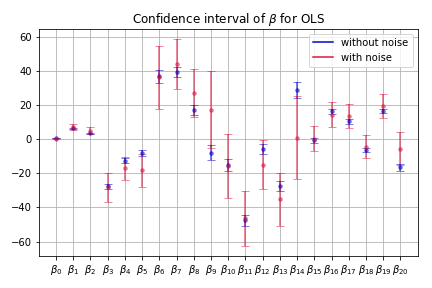
\includegraphics[width=0.6\linewidth]{confIntBeta_OLS.png}
	\caption{This is a plot of the 98\% confidence intervals of the regression parameters $\beta$ for the OLS model. The blue dots/lines indicate the confidence intervals for the Franke function without noise, while the red indicates the confidence intervals with noise ($\sigma=0.2$). As we see even with a small noise added, the confidence intervals can be quite large. By following the link in Appendix \ref{sect:appendix} to GitHub, we can see a plot for the confidence intervals for $\sigma=1$, and they are much much bigger than what we got here.\label{fig:conf_int_OLS}}
\end{figure} 

\begin{figure}[htbp]
	\centering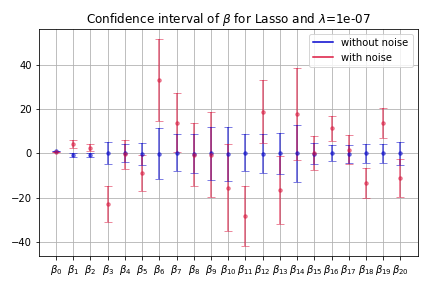
\includegraphics[width=0.6\linewidth]{confIntBeta_Lasso_1e-07.png}
	\caption{This is a plot of the 98\% confidence intervals of the regression parameters $\beta$ for the Lasso model with $\lambda=10^{-7}$. Here we see the blue for the Franke function without noise laying more ore less on zero, while the red noise is a little more scattered above and belove zero.\label{fig:conf_int_Lasso}}
\end{figure} 

Now we look at the results we get when we introduce the k-fold cross-validation resampling on the regression methods. In figure \ref{fig:biasvar_OLS} we see the bias-variance tradeoff for the OLS model with resampling for 5 folds.

\begin{figure}[htbp]
	\centering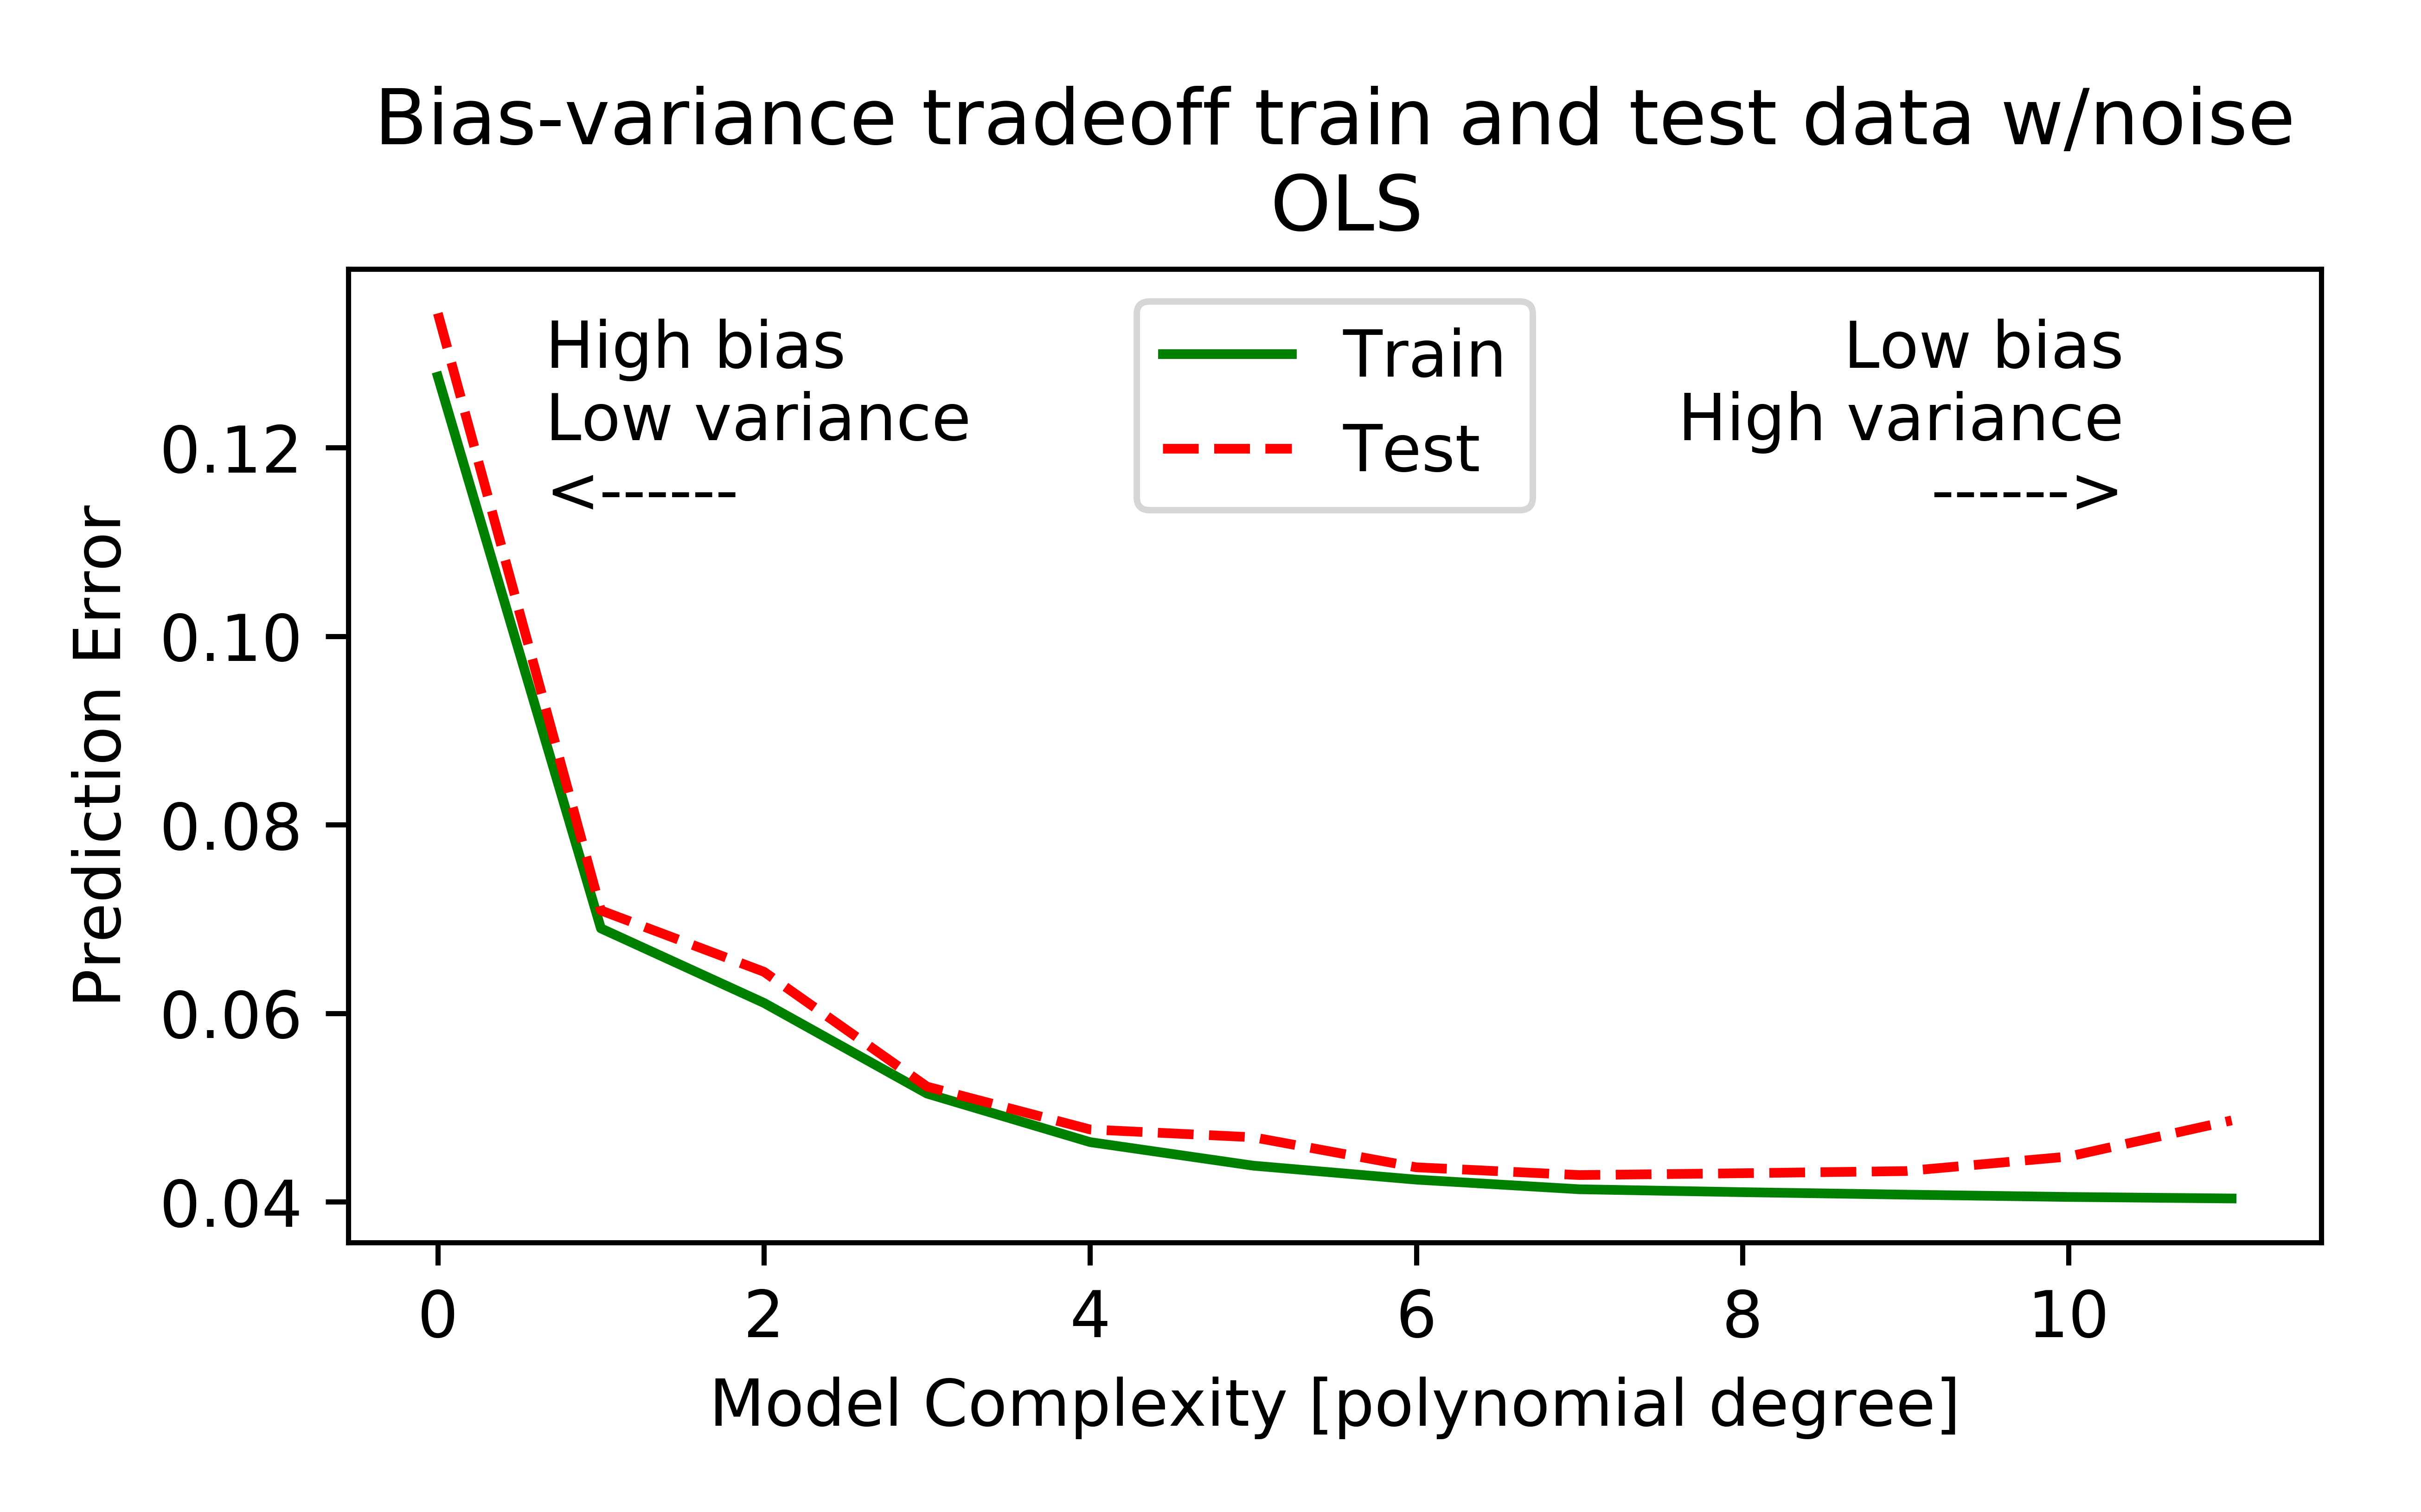
\includegraphics[width=0.6\linewidth]{biasvariancetradeoff_OLS_Franke_noise.png}
	\caption{In this figure we see the bias-variance tradeoff for increasing model complexity for the prediction error (MSE) for training and test data of the Franke function with noise.This is for the OLS model with k-fold cross-validation resampling with 5 folds. When the model complexity is getting higher, around 8-9, we see that the test curve starts to increase more. This comes from overfitting. In this figure we have included the regions of the variance and the bias as well, but these can be individually seen in Figure \ref{fig:var_bias}.\label{fig:biasvar_OLS}}
\end{figure} 

\begin{figure}[htbp]
	%\hspace*{-2.5cm}
	\subfloat[Plot of the variance of the data with OLS and resampling ]{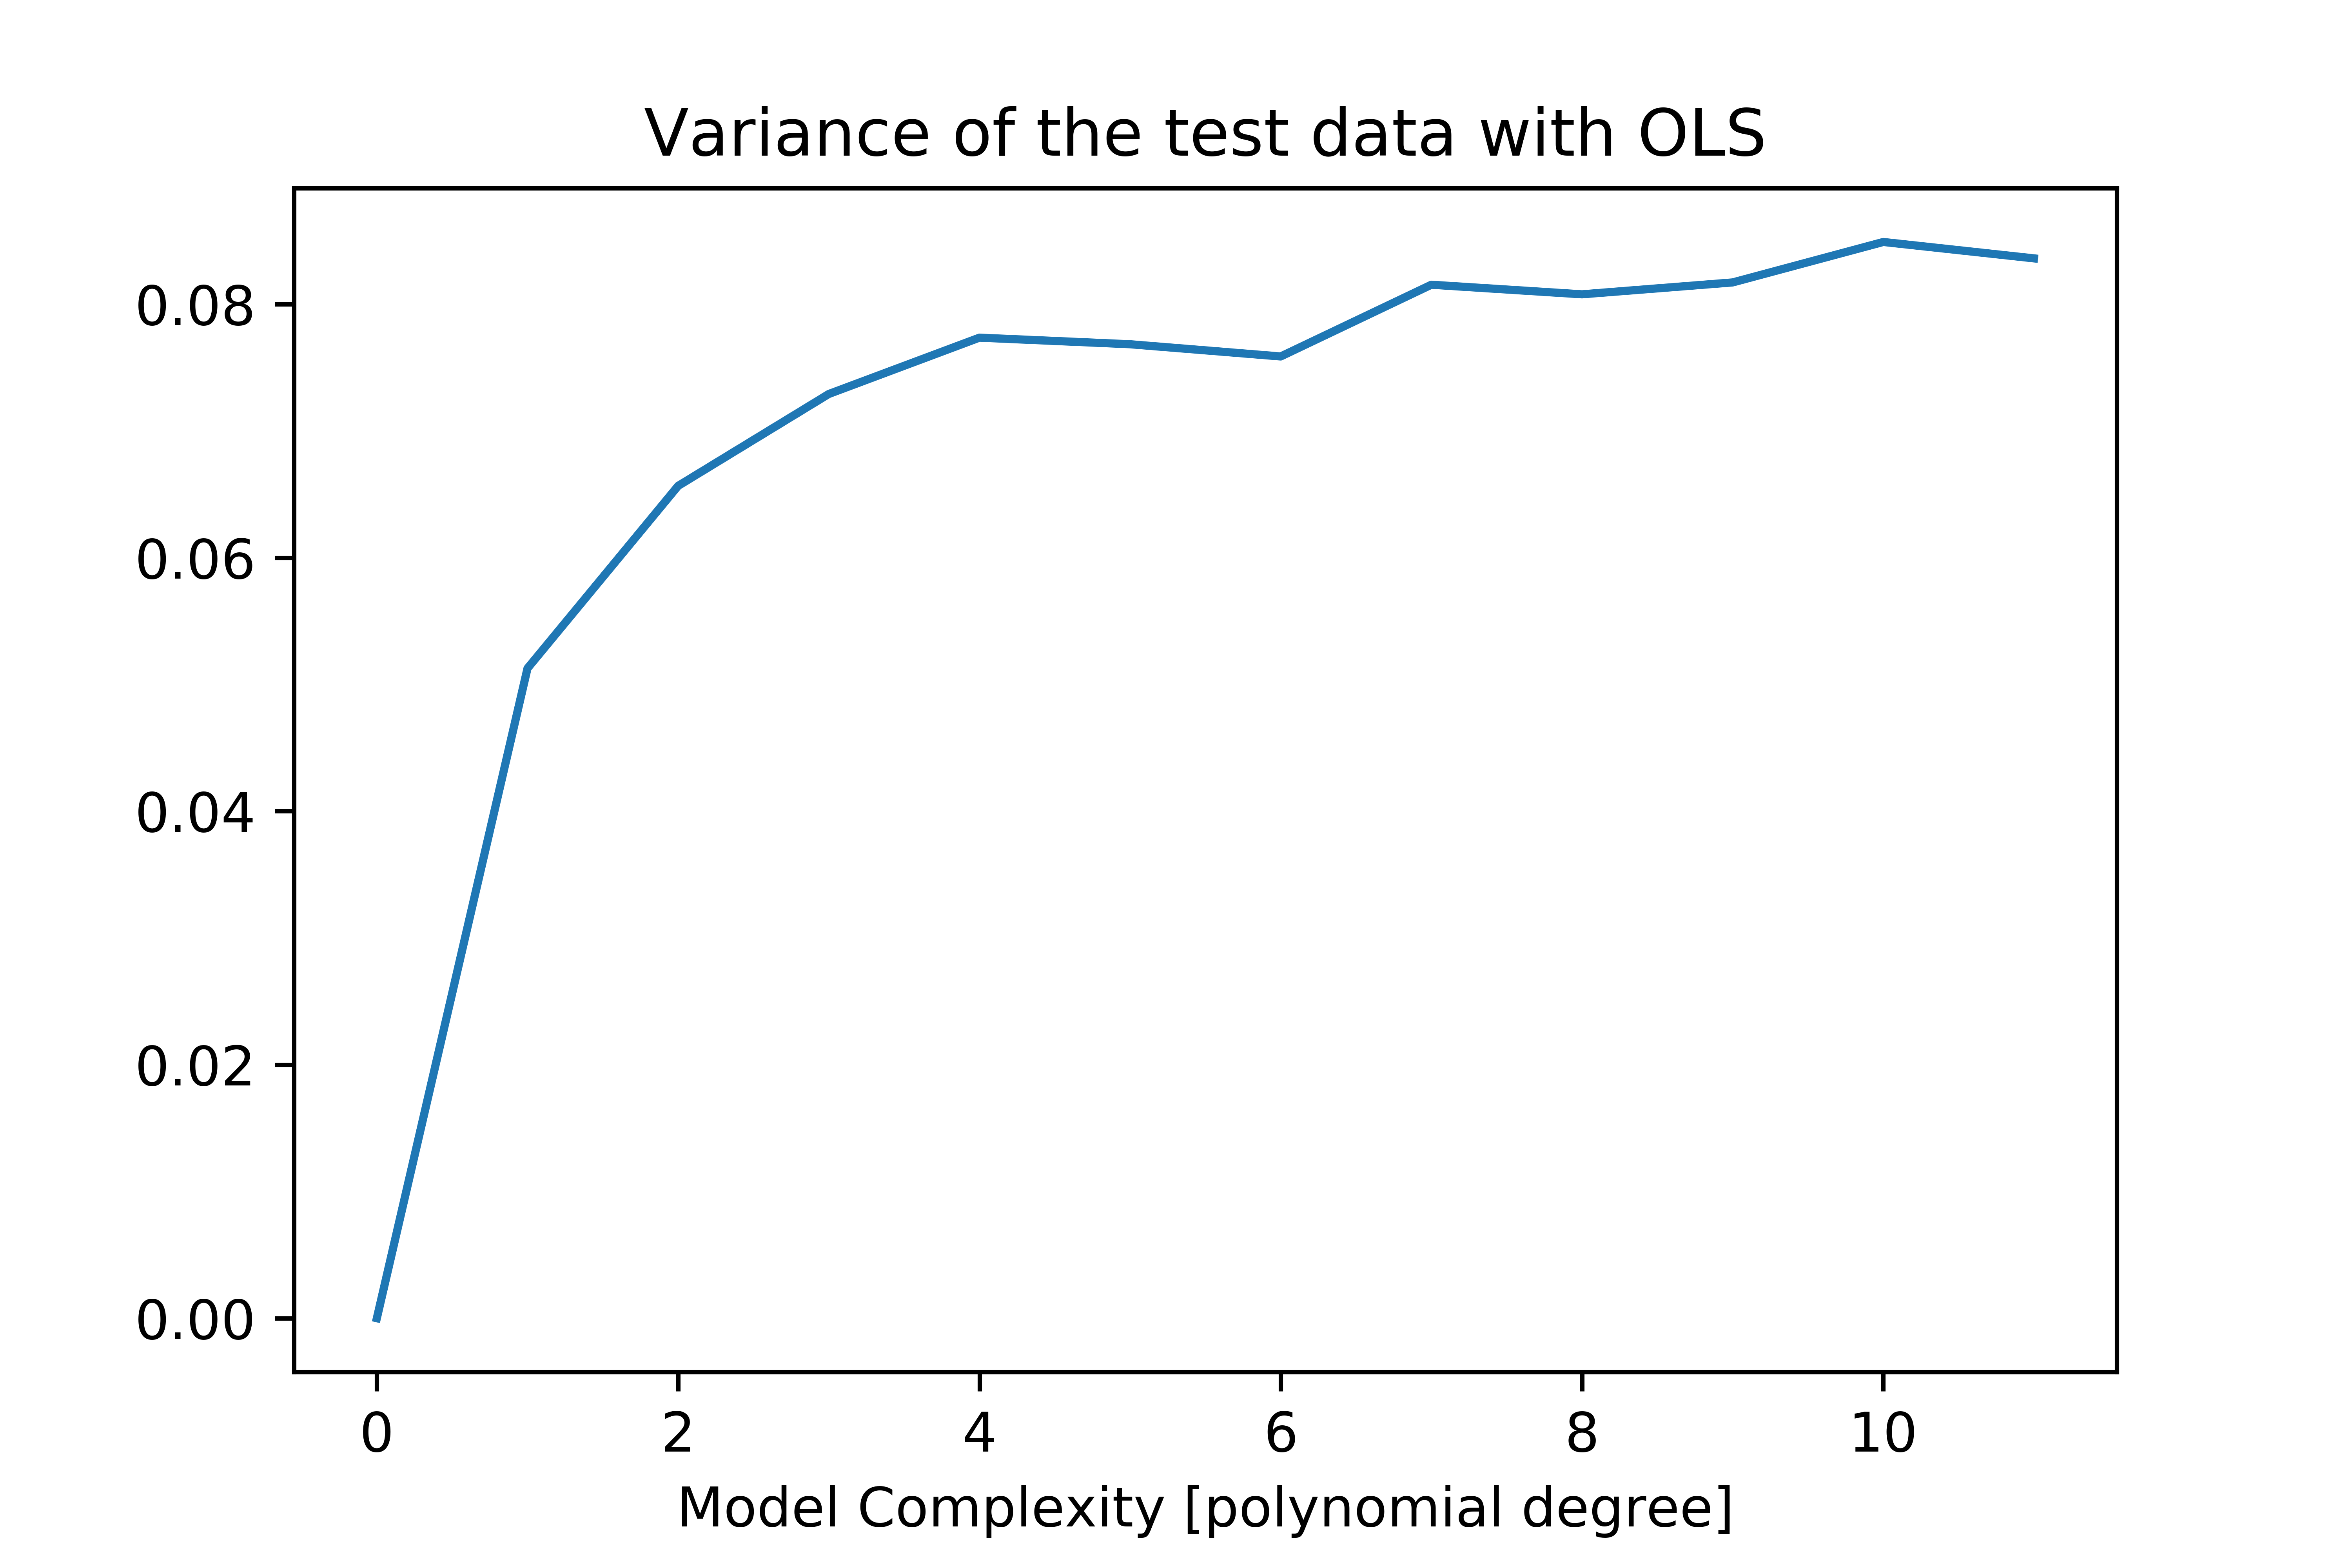
\includegraphics[width=0.5\linewidth]{biasvar_Var_OLS.png}}
	\subfloat[Plot of the bias of the data with OLS and resampling ]{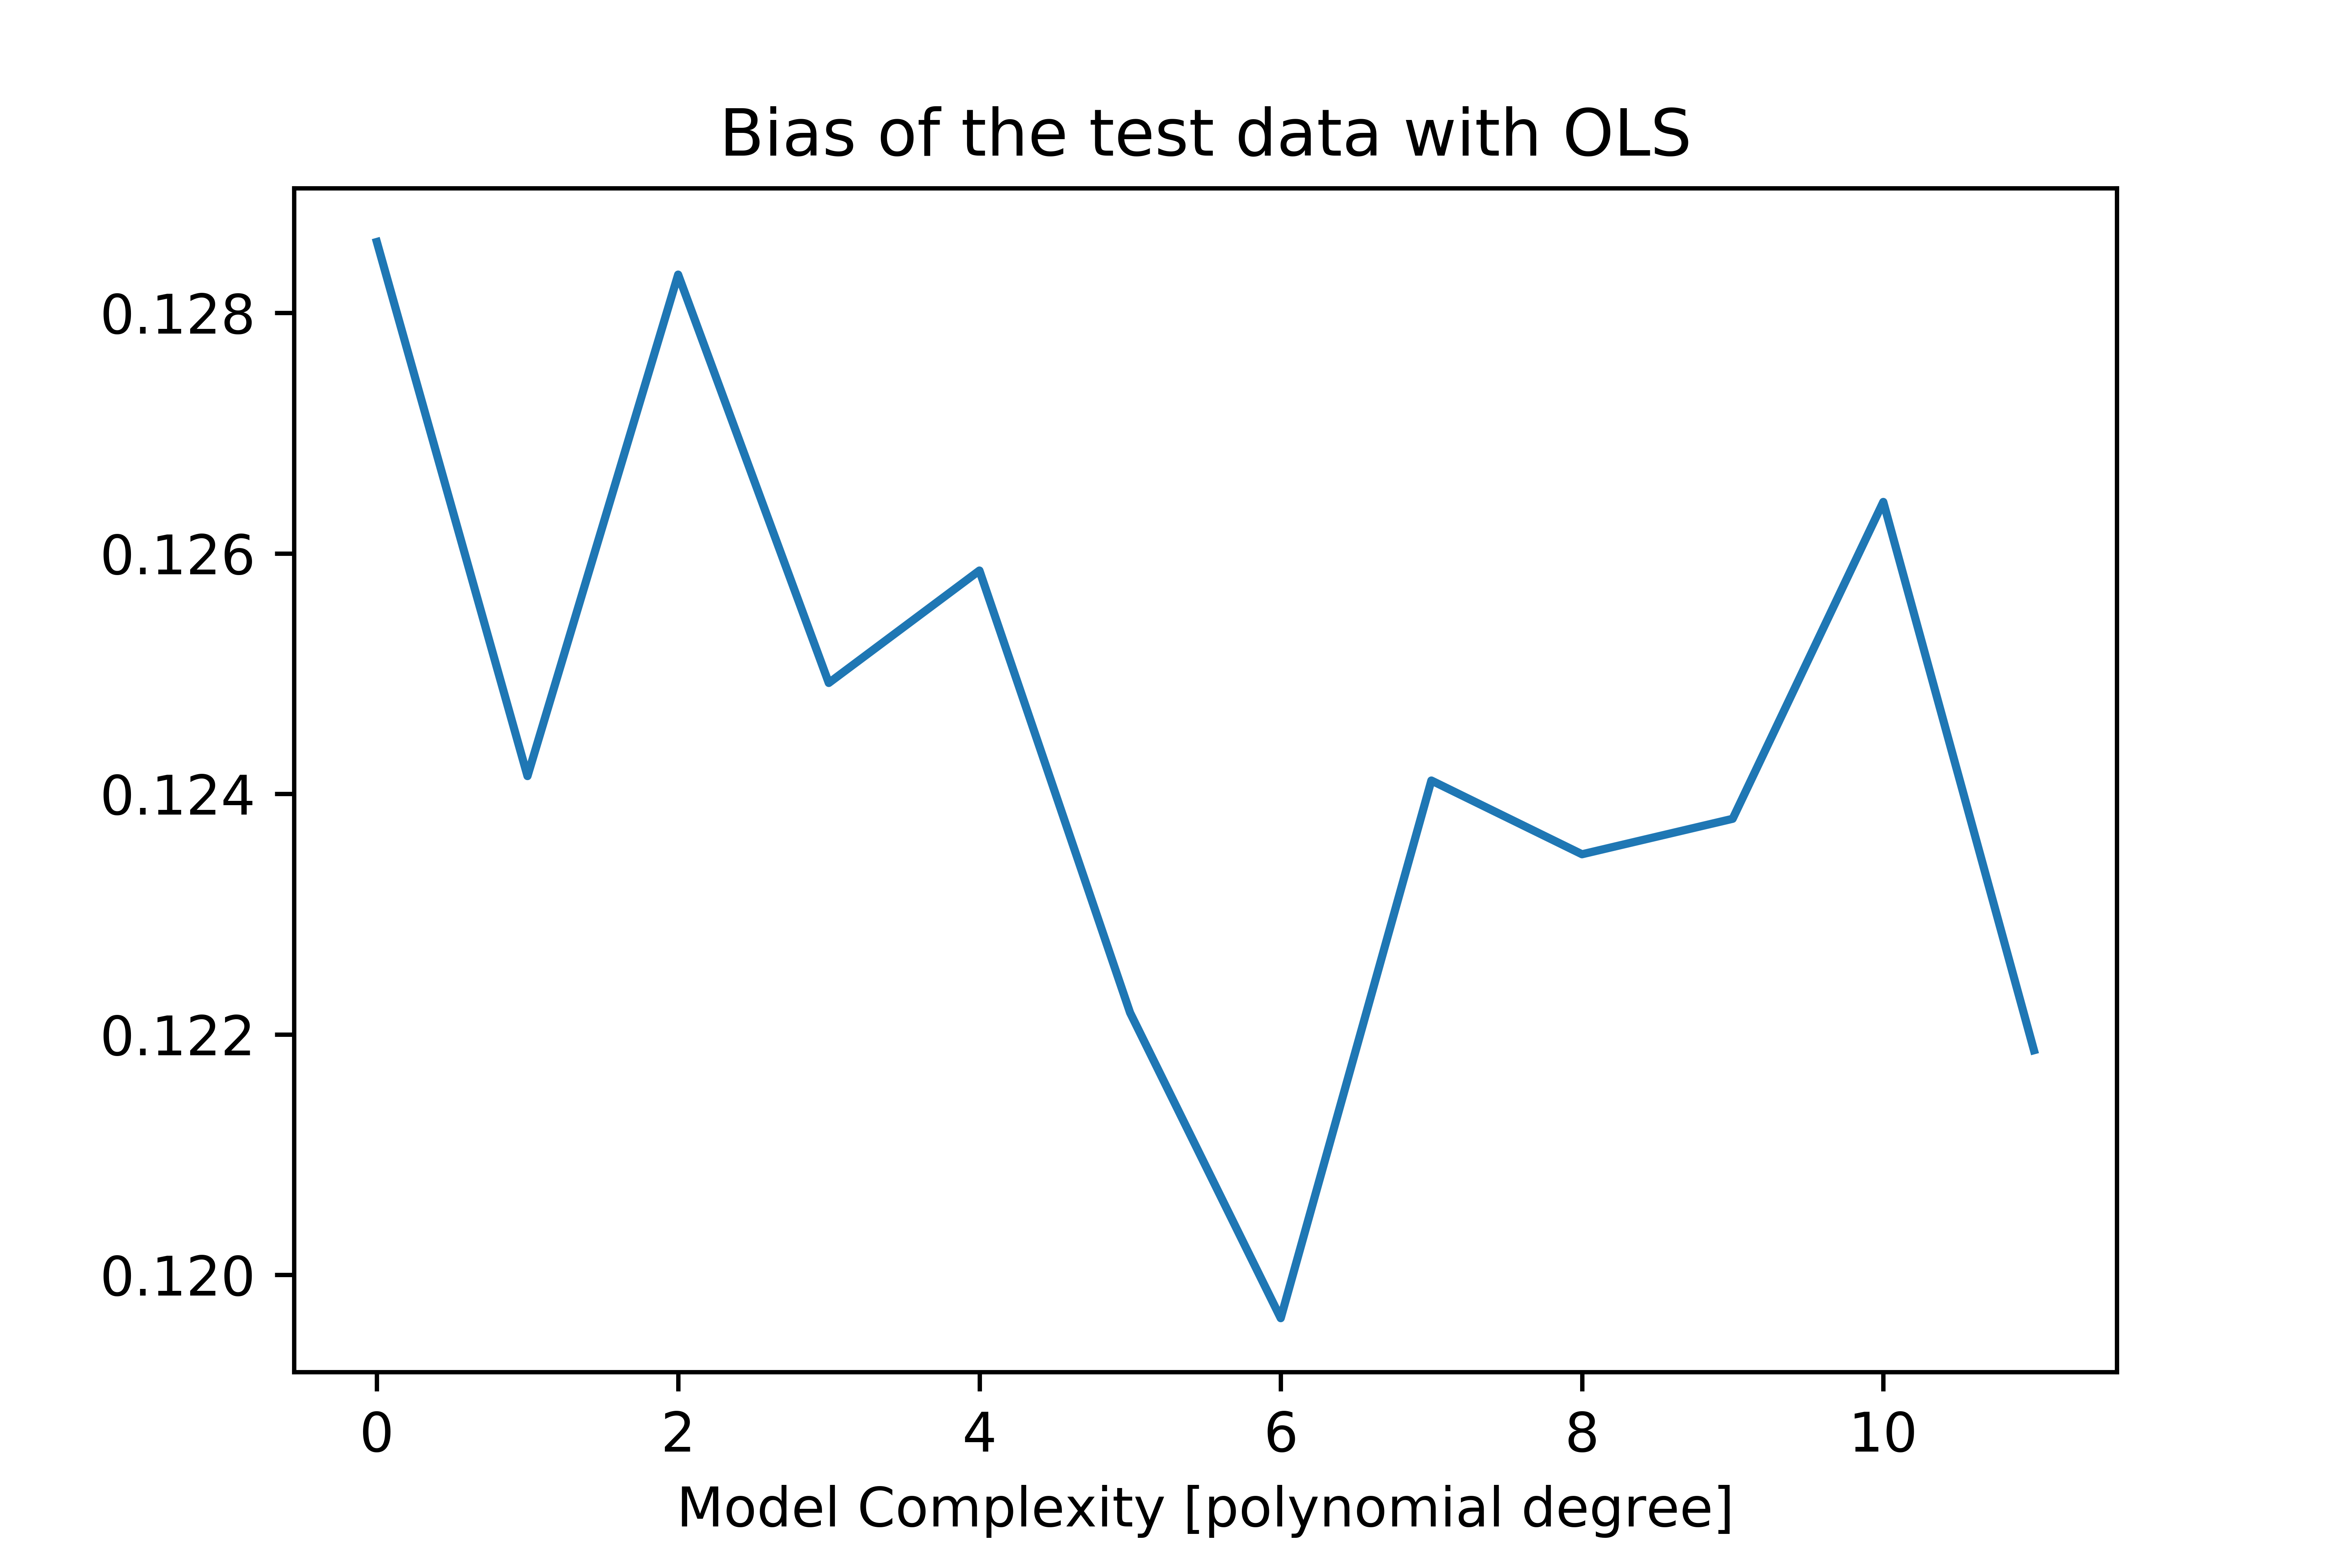
\includegraphics[width=0.5\linewidth]{biasvar_Bias_OLS.png}}
	\caption{Here we see how the variance and bias behave for increasing model complexity for the Franke function with the OLS model and resampling. As expected for the OLS model, the variance increases with the model complexity, while the bias (somewhat) decreases. This is the core of bias-variance tradeoff where they are dependent on each other, so if one increases then the other decreases. We also see that there is a much higher change in the variance than in the bias.\label{fig:var_bias}}
\end{figure}


\subsection{Digital data}
\section{Conclusion}

\appendix
\section{Appendix}
\label{sect:appendix}
Link to GitHub repository:\\

\section{Appendix}
\label{sect:bias_var_calc}
The full calculation of the rewritten cost function from equation \ref{eq:cost_func} to the bias-variance tradeoff equation \ref{eq:bias_var}:\\
We start by using that $\textbf{y}=f(\textbf{x})+\hat{\epsilon}$ and $\tilde{\textbf{y}}=\textbf{X}\hat{\beta}$.
\begin{align*}
\mathds{E}[(\textbf{y}-\tilde{\textbf{y}})^2]&=\mathds{E}[(\textbf{f}+\hat{\epsilon}-\tilde{\textbf{y}})^2]= \mathds{E}[(\textbf{f}+\hat{\epsilon}-\tilde{\textbf{y}}+\mathds{E}[\tilde{\textbf{y}}]-\mathds{E}[\tilde{\textbf{y}}])^2]\\
&=\mathds{E}[(\textbf{f}^2-2\textbf{f}\mathds{E}[\tilde{\textbf{y}}]+\mathds{E}[\tilde{\textbf{y}}]^2)+(\tilde{\textbf{y}}^2-2\tilde{\textbf{y}}\mathds{E}[\tilde{\textbf{y}}]+\mathds{E}[\tilde{\textbf{y}}]^2)+\mathds{E}[\hat{\epsilon}^2]]
\end{align*}
Here we have used that the expectation value of $\hat{\epsilon}$ is $\mathds{E}[\hat{\epsilon}]=0$, and that the expectation value of $\tilde{\textbf{y}}$ is $\mathds{E}[\tilde{\textbf{y}}]=\textbf{X}\hat{\beta}$ \cite{hastie2009}\footnote{Chapter 7.3 - equation (7.9)}. Then we split the equation such that we get:
\begin{align*}
\mathds{E}[(\textbf{y}-\tilde{\textbf{y}})^2]=\mathds{E}[(\textbf{f}-\mathds{E}[\tilde{\textbf{y}}])^2]+\mathds{E}[(\tilde{\textbf{y}}-\mathds{E}[\tilde{\textbf{y}}])^2]-\mathds{E}[\hat{\epsilon}^2]
\end{align*}
Now we use that the expectation value of $\hat{\epsilon}^2$ is $\mathds{E}[\hat{\epsilon}^2]=Var[\textbf{y}]=\sigma^2$ since $\mu=0$. The other expectation values can be discretized in terms of sums as:
\begin{equation*}
\mathds{E}[(\textbf{y}-\tilde{\textbf{y}})^2]=\frac{1}{n}\sum_{i}(f_i-\mathds{E}[\tilde{\textbf{y}}])^2+ \frac{1}{n}\sum_{i}(\tilde{y}_i-\mathds{E}[\tilde{\textbf{y}}])^2+\sigma^2
\end{equation*}

\bibliographystyle{plainnat}
\bibliography{myrefs}
\end{document}